\chapter{Zadanie problému a cieľové požiadavky}

\section{Úvodné definície a značenia}
Na začiatok si zaveďme niektoré dôležité pojmy z teórie grafov.
Budú sa týkať obecnej teórie a úlohu so všetkými jej špecifikami si ozrejmíme v nasledujúcej kapitole.
\begin{define}
{\sl Graf G} je usporiadaná dvojica (V, E), kde V označuje množinu vrcholov(vertices) a $E \subseteq V \times V $ označuje množinu hrán (edges). Značíme G = (V, E).
\end{define}

\begin{define}
{\sl Ohodnotený graf (G, w)} je graf s spolu s reálnou funkciou (tzv. ohodnotením)
$w: E(G) \to \R$, kde $w$ je funkcia, ktorá každej hrane priradí
reálne číslo, takzvanú \emph{cenu}, alebo \emph{dĺžku} hrany.
\end{define}
ukazka na \ref{fig:ohodnoteny_graf}

\begin{figure}[h]
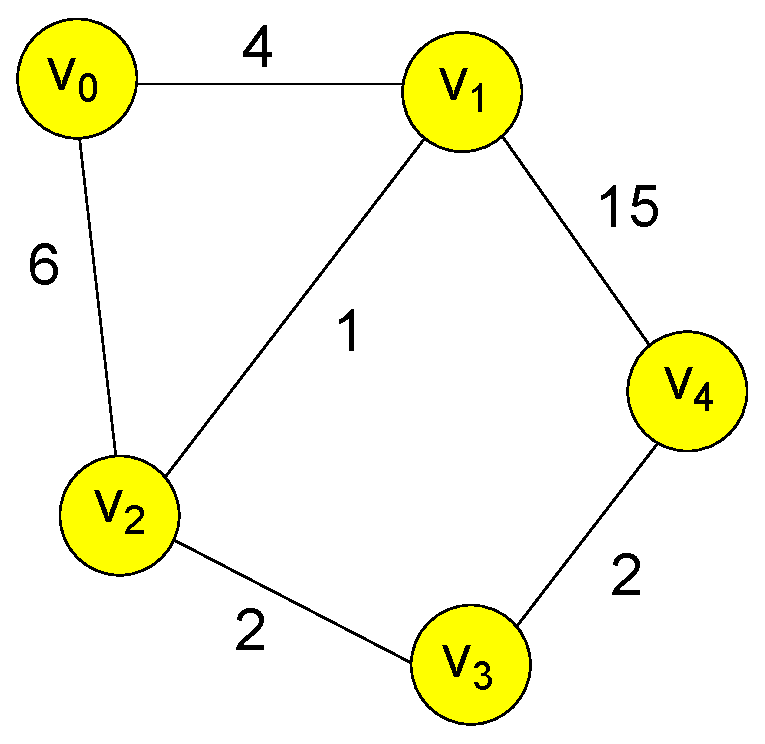
\includegraphics[height=7.5cm]{./img/graf.eps}
\caption{Ohodnotený graf}
\label{fig:ohodnoteny_graf}
\end{figure}

Teraz keď už vieme, čo je to graf, skúsme si zadefinovať najkratšiu cestu. Začnime najprv obecne cestou.

\begin{define}
{\sl Cesta P z vrcholu $v_0$ do vrcholu $v_n$ v grafe G } je postupnosť $P = (v_{0},e_{1},v_{1},\dots, e_{n}, v_{n})$,
pre ktorú platí $e_{i} = \{v_{i-i},v_{i}\}$ a taktiež
$v_{i} \ne v_{j}$ pre každé $i \ne j$.
\end{define}






Všimnime si, že v ceste nenavštívime žiaden vrchol dvakrát a teda cesta neobsahuje kružnice.

TODO?? dlzka hrany - cena cesty - zadefinuj funkciu d(u, v)

\begin{define}
{\sl Cena cesty P z vrcholu $v_0$ do vrcholu $v_n$ v ohodnotenom grafe (G, w) } je súčet cien hrán, ktoré sa na ceste nachádzajú.
\end{define}

\begin{define}
{\sl Najkratšia cesta P z vrcholu $v_0$ do vrcholu $v_n$
v ohodnotenom grafe (G, w)} 
je cesta s najnižsou cenou.
\end{define}





\section{Mriežkový graf}

Po zavedení kľúčových pojmov sa dostávame k samotnému zadaniu úlohy. 
Ako sme už spomínali, problém budeme riešit na tzv. mriežkových grafoch. Čo je mriežkový graf a v čom sa od obecného grafu odlišuje?

Zjednodušene povedané, je to mapa s ktorou sa stretávame v najrôznejších hrách, ako je Warcraft, Startcraft, Dragon Age
a~podobne. ASK?? je to "mapa" dat do uvodzoviek

Ide o špeciálny a dosť obmedzený typ grafu. Vizuálne si ho môžme predstaviť ako konečný graf v ktorom sú vrcholy rozostúpené v tvare mriežky a hrana
je stále medzi dvojicami susedných vrcholov vo všetkých ôsmych smeroch. Cena vodorovnej alebo zvislej hrany je $1$ a cena šikmej hrany je $\sqrt{2}$.


\begin{figure}[h]
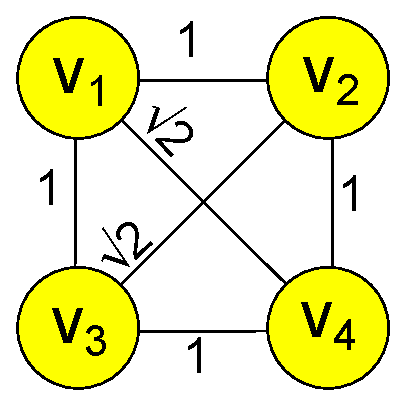
\includegraphics[height=5.5cm]{./img/herna_mapa2x2.eps}
\caption{Mriežkový graf 2x2}
\label{fig:mriezkovy_graf2x2}
\end{figure}


\begin{figure}[h]
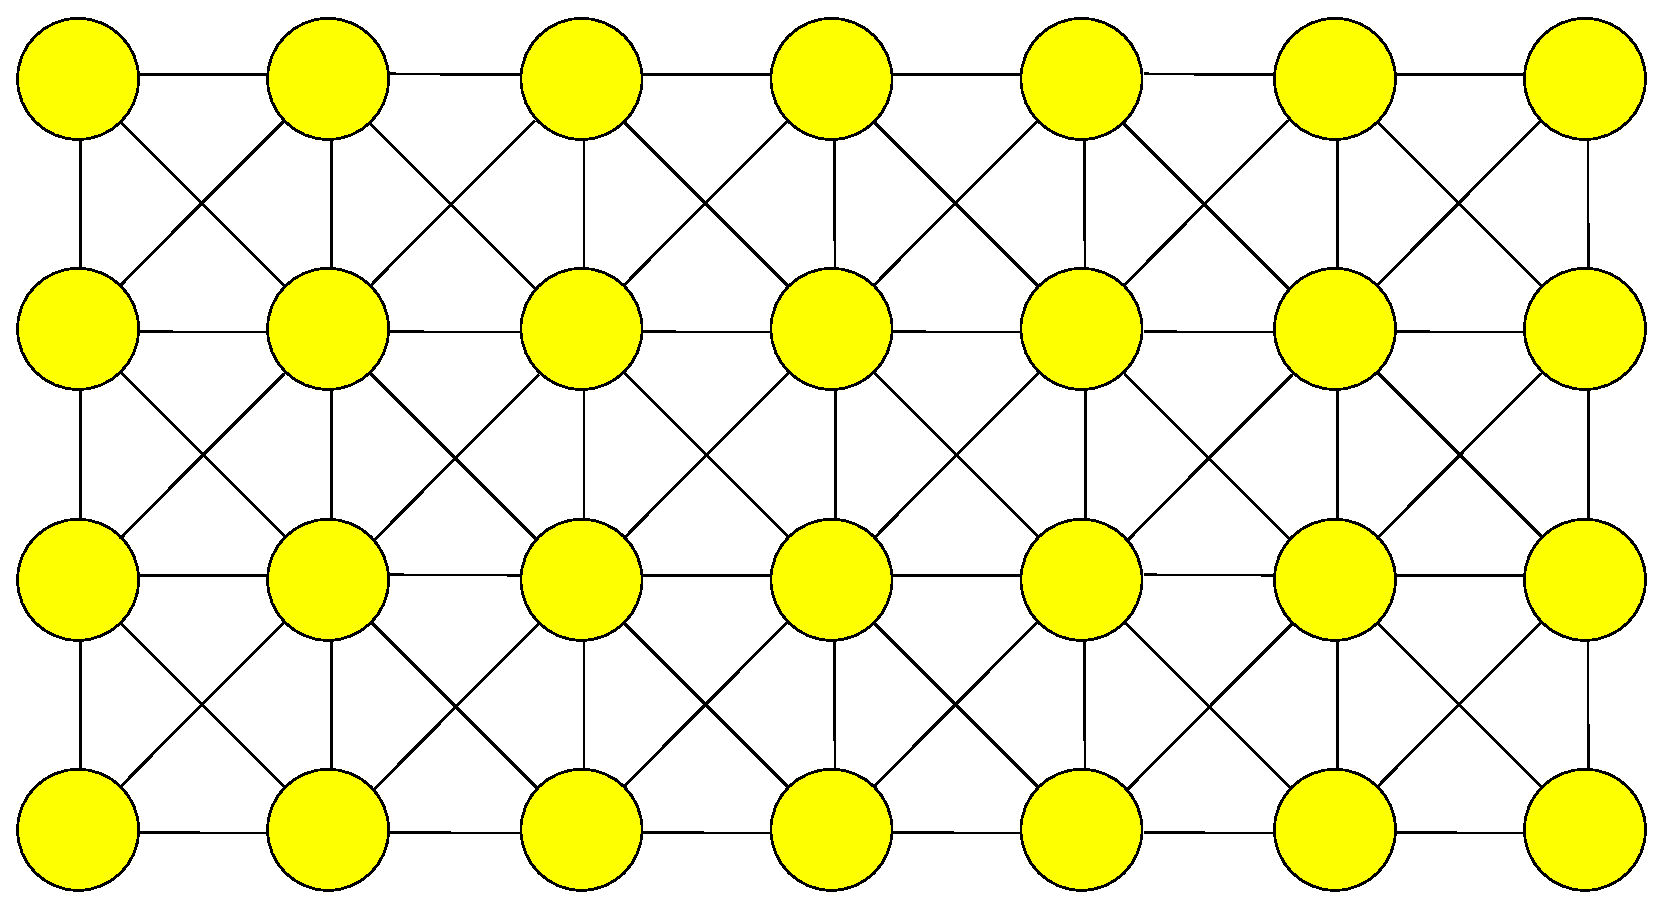
\includegraphics[height=5.5cm]{./img/herna_mapa.eps}
\caption{Mriežkový graf bez označenia vrcholov a dĺžok hrán}
\label{fig:mriezkovy_graf}
\end{figure}


Zadefinujme si teraz mriežkový graf formálne.

\begin{define}
{\sl Mriežkový graf rozmerov m*n} je ohodnotený graf v ohodnotením $w$ s m*n vrcholmi očíslovanými od $v_{1,1}$ až po $v_{m,n}$ 
s~jednoduchými hranami $j$ v~tvare $\{v_{a,b}, v_{a,b+1}\}, \{v_{a,b}, v_{a+1,b}\}$, kde $w(j) = 1$ 
a šikmými hranami $ s $ v~tvare 
$\{v_{a,b}, v_{a+1,b+1}\}$, $\{v_{a,b}, v_{a+1,b+1}\}$, kde $ w(s) = \sqrt{2}$.
\end{define}

FIXME?? pridat obrazky

\begin{note}
	Mriežkový graf sa dá reprezentovať ako matica m*n nad telesom $\Z_2$, kde jednotky predstavujú vrcholy. Príklad maticovej reprezentácie grafu rozmerov 4x5 je na obrázku
	\ref{fig:maticova_reprezentacia}.
\end{note}



\begin{figure}[h]
\caption{Maticová reprezentácia mriežkového grafu}
\label{fig:maticova_reprezentacia}
\[
G =
  \begin{bmatrix}
    0 & 0 & 1 & 1 & 1 & 1\\
	0 & 0 & 1 & 1 & 1 & 0\\
	0 & 0 & 0 & 1 & 1 & 1\\
	0 & 0 & 0 & 0 & 0 & 0\\
  \end{bmatrix}
\]
\end{figure}




\section{GPPC: Grid-Based Path Planning Competition}
Algoritmus navrhnutý a naprogramovaný v tejto práci bol zaradený do súťaže \textbf{GPPC}, ktorá sa koná približne 2 krát ročne.

\subsection{Špecifiká súťaže, limity}

Herné mapy budú mať rozmery maximálne $2048 \times 2048$.
Súťaž bude rozdelená do dvoch fáz --- fázy predspracovania mapy(pre-processing)
a fázy testovania. Na predspracovanie mapy bude vyhradený čas
maximálne 30 minút a program si svoje dáta uloží na disk do súboru o veľkosti maximálne 50MB.
A potom vo fáze testovania budé dostávať požiadavky na nájdenie najkratšej cesty.

Úlohou súťaže je naimplementovať tieto tri funkcie.

\lstset{language=C++}          % Set your language (you can change the language for each code-block optionally)

\begin{lstlisting} %[frame=single]  % Start your code-block

void PreprocessMap(std::vector &bits, int width, int height,
                   const char *filename);
                   
void *PrepareForSearch(std::vector &bits, int width, int height,
                       const char *filename);
bool GetPath(void *data, xyLoc s, xyLoc g, std::vector &path);
\end{lstlisting}

\subsection{Kritériá súťaže, hodnotenie programov}
Programy sa nebudú porovnávať v jednej metrike a podľa jedného
kritéria, nakoľko sa programy dalo zoptimalizovať podľa viacerých kritérií. Metriky sú nasledovné:

\begin{itemize}
\item Celkový čas na~nájdenie cesty.
\item Čas na nájdenie prvých 20 tich krokov.
\item Dĺžka cesty (zohľadnená suboptimalita).
\item Maximálny čas vrátenia hociktorej časti cesty.
\end{itemize}

Testovací počítač má 12 GB RAM pamäti a dva 2.4 Ghz Intel Xeon E5620
procesory.